\everymath{\displaystyle}
\documentclass{beamer}
% \documentclass[handout]{beamer}

%\usepackage[pdftex]{color,graphicx}
\usepackage{amsmath,amssymb,amsfonts}

\mode<presentation>
{
  % \usetheme{Darmstadt}
  % \usetheme[hideothersubsections]{Hannover}
  % \usetheme[hideothersubsections]{Goettingen}
  \usetheme[hideothersubsections, right]{Berkeley}

  \usecolortheme{seahorse}
  % \usecolortheme{dolphin}
  \usecolortheme{rose}
  % \usecolortheme{orchid}

  \useinnertheme[shadow]{rounded}

  \setbeamercovered{transparent}
  % or whatever (possibly just delete it)
}

\mode<handout>{
  \setbeamercolor{background canvas}{bg=black!5}
  \usepackage{pgfpages}
  \pgfpagesuselayout{4 on 1}[a4paper,border shrink=5mm, landscape]
}

\usepackage[brazilian]{babel}
% or whatever

% \usepackage[latin1]{inputenc}
\usepackage[utf8]{inputenc}
% or whatever

\usepackage{times}
%\usepackage[T1]{fontenc}
% Or whatever. Note that the encoding and the font should match. If T1
% does not look nice, try deleting the line with the fontenc.


\title%[] % (optional, use only with long paper titles)
{Problema, Hipóteses e Variáveis}

\subtitle
{} % (optional)

\author%[] % (optional, use only with lots of authors)
{Felipe Figueiredo}% \and S.~Another\inst{2}}
% - Use the \inst{?} command only if the authors have different
%   affiliation.

\institute[INTO] % (optional, but mostly needed)
{Instituto Nacional de Traumatologia e Ortopedia
}
  % \inst{1}%
  % Department of Computer Science\\
  % University of Somewhere
  % \and
  % \inst{2}%
  % Department of Theoretical Philosophy\\
  % University of Elsewhere}
% - Use the \inst command only if there are several affiliations.
% - Keep it simple, no one is interested in your street address.

\date%[] % (optional)
{}

% \subject{Talks}
% This is only inserted into the PDF information catalog. Can be left
% out. 



% If you have a file called "university-logo-filename.xxx", where xxx
% is a graphic format that can be processed by latex or pdflatex,
% resp., then you can add a logo as follows:

\pgfdeclareimage[height=1.6cm]{university-logo}{../logo}
\logo{\pgfuseimage{university-logo}}



% Delete this, if you do not want the table of contents to pop up at
% the beginning of each subsection:
\AtBeginSubsection[]
%\AtBeginSection[]
{
  \begin{frame}<beamer>{Sumário}
    \tableofcontents[currentsection,currentsubsection]
  \end{frame}
}


% If you wish to uncover everything in a step-wise fashion, uncomment
% the following command: 

% \beamerdefaultoverlayspecification{<+->}


\begin{document}

\begin{frame}
  \titlepage
\end{frame}

\begin{frame}{Sumário}
  \tableofcontents
  % You might wish to add the option [pausesections]
\end{frame}


%% Template
% \section{}

% \subsection{}

% \begin{frame}{}
%   \begin{itemize}
%   \item 
%   \end{itemize}
% \end{frame}

% \begin{frame}
%   \begin{columns}
%     \begin{column}{5cm}
%     \end{column}
%     \begin{column}{5cm}
%     \end{column}
%   \end{columns}
% \end{frame}

% \begin{frame}{}
%   \includegraphics[height=0.4\textheight]{file1}
%   \includegraphics[height=0.4\textheight]{file2}
%   \includegraphics[height=0.4\textheight]{file3}
%   \begin{figure}
%     \caption{}
%   \end{figure}
% \end{frame}

% \begin{frame}{}
%   \begin{definition}
%   \end{definition}
%   \begin{example}
%   \end{example}
%   \begin{block}{Exercício}
%   \end{block}
% \end{frame}

\section{Discussão da aula passada}

\subsection{Discussão da aula passada}

\begin{frame}{Discussão da aula passada}
  \begin{block}{}
    Discussão da leitura obrigatória da aula passada
  \end{block}
\end{frame}

\section{Problema}

\begin{frame}{Problema de pesquisa}
  \begin{itemize}
  \item Questão não resolvida, lacuna no conhecimento
  \item Assunto que se precisa provar ou desenvolver
  \item Vinculado (e restrito) a um Tema
  \item Nosso ``ganha-pão''
  \end{itemize}
\end{frame}

\begin{frame}{Exemplo}
  \begin{example}
    Tema: ``O perfil da mãe que deixa o filho para adoção''

    \bigskip

    Problema: ``Quais condições exercem mais influência na decisão das
    mães em dar o filho recém-nascido para adoção?''
  \end{example}
  Lakatos, Marconi (2003)
\end{frame}

\begin{frame}{Tema x Problema x Hipótese}
  \begin{itemize}
  \item Tema: assunto
  \item Problema: pergunta
  \item Hipótese: resposta provisória
  \end{itemize}
\end{frame}

\begin{frame}
  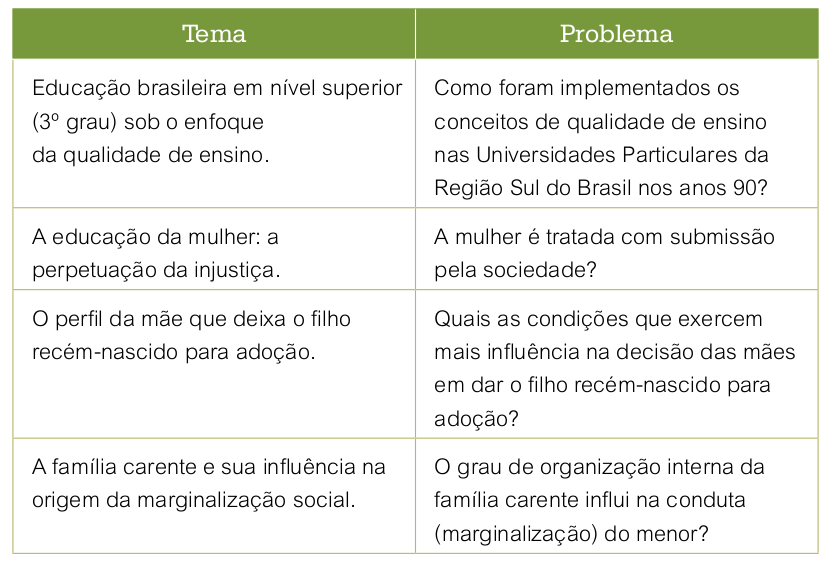
\includegraphics[height=0.8\textheight]{Hipoteses_variaveis/tema_problema}

  Fonte: Prodanov, 2013
\end{frame}

\begin{frame}{Formulação do Problema}
O problema é:
  \begin{itemize}
  \item original?
  \item relevante?
  \item viável (recursos, tempo, etc)?
  \end{itemize}
Prodanov, 2013
\end{frame}

\section{Hipóteses}

% \subsection{Hipóteses}

\begin{frame}{Hipóteses}
  \begin{block}{}
    ``(...) um enunciado geral de \alert{relações entre variáveis}
    (fatos, fenômenos).''

\bigskip

Lakatos, Marconi (2003)
  \end{block}
  % \begin{itemize}
  % \item Solução provisória para o problema
  % \item Caráter explicativo ou preditivo
  % \item Compatível com conhecimento científico (coerência externa)
  % \item Consistência lógica (coerência interna)
  % \item Empiricamente verificável
  % \end{itemize}
  \begin{block}{}
    ``(...) constituem ``respostas'' supostas e provisórias ao
    problema. A principal resposta é denominada hipótese básica,
    podendo ser complementada por outras (...) secundárias.''

    \bigskip
    Prodanov, 2013
  \end{block}
\end{frame}

\begin{frame}{Hipóteses}
  \begin{itemize}
  \item Declaração que antecipa a relação entre duas ou mais variáveis
  \item Problema, pesquisa e hipótese estão relacionados
  \item Deduzida da revisão bibliográfica
  \item Em estudos quantitativos, pode ser testada (Estatística!)
  \item É uma ``aposta'' que o pesquisador faz sobre os possíveis
    resultados
  \end{itemize}
  (Fonte: Prodanov, 2013)
\end{frame}

\begin{frame}{Características das hipóteses}
  \begin{itemize}
  \item Consistência lógica
  \item Simplicidade (Navalha de Occam)
  \item Verificabilidade
  \item Embasamento teórico
  \item Especificidade
  \item Plausibilidade
  \item Originalidade
  \end{itemize}
  (Fonte: Prodanov, 2013)
\end{frame}

\begin{frame}{Navalha de Occam}
  \begin{definition}
    {\em entia non sunt multiplicanda praeter necessitatem}

    \bigskip
    entidades não devem ser multiplicadas sem necessidade
  \end{definition}
  \begin{itemize}
  \item William of Ockham (1287 -- 1347)
  \item ``Lei da parcimônia'' ({\em Lex Parsimoniae})
  \item Elegância na simplicidade
  \end{itemize}
\end{frame}
\begin{frame}{Fontes de hipóteses}
  As hipóteses tipicamente surgem de
  \begin{itemize}
  \item Observação
  \item Resultados de outras pesquisas
  \item Teorias
  \item Intuição
  \end{itemize}
  (Fonte: Prodanov, 2013)
\end{frame}

\begin{frame}{Formulação de hipóteses}
Atenção: Hipóteses não são perguntas, e sim afirmações

\begin{example}
  Problema: como o Marketing de patrocínio contribui no processo de
  construção da marca das organizações?

  \begin{itemize}
  \item organizações que patrocinam causas éticas, ambientais e
    sociais possuem melhoria de imagem e crescimento de vendas junto à
    comunidade
  \item o marketing de patrocínio fortalece o envolvimento dos
    funcionários com a missão da empresa.
  \end{itemize}
  Prodanov, 2013
\end{example}
\end{frame}

\section{Variáveis}

\begin{frame}{Variáveis}
  \begin{itemize}
  \item Hipóteses também podem ser formuladas como uma conexão causal
    entre duas (ou mais) variáveis
  \item Se X, então Y
  \item Variáveis podem
    \begin{itemize}
    \item descrever o fenômeno
    \item explicar o fenômeno
    \end{itemize}
  \end{itemize}
\end{frame}

\begin{frame}{Tipos de Variáveis}
  \begin{definition}
    Variável \alert{dependente} (ou resposta) é a variável a ser
    explicada no estudo.
  \end{definition}
  \begin{definition}
    Variável \alert{independente} (ou explanatória) é a variável que
    serve de suporte na explicação da variabilidade da variável
    resposta.
  \end{definition}
\end{frame}

\subsection{Níveis de mensuração}

\begin{frame}{Tipos de Variáveis}
Variáveis podem ser classificadas em duas principais categorias
  \begin{itemize}
  \item Qualitativas (categóricas)
  \item Quantitativas (numéricas)
  \end{itemize}
  \begin{example}
    Pressão sistólica (mmHg), altura (cm), sexo (M ou F), grau de
    satisfação com atendimento médico (nota de 1 a 5), perímetro
    abdominal (cm), contagem de leucócitos, número de pessoas na
    família, cor da pele (branco, negro, pardo), etc.
  \end{example}
\end{frame}

\begin{frame}{Variáveis qualitativas}
Variáveis qualitativas se subdividem em
  \begin{itemize}
  \item<1-2> Nominais
  % \begin{example}
  %   sexo, cor da pele
  % \end{example}

  \item<3-4> Ordinais
  \end{itemize}

  % \begin{example}
  %   satisfação com atendimento médico (nota de 1 a 5)
  % \end{example}

  \begin{example}
    Pressão sistólica (mmHg), altura (cm), \only<2>\alert{sexo (M ou
      F)}, \only<4>\alert{grau de satisfação com atendimento médico
      (nota de 1 a 5)}, perímetro abdominal (cm), contagem de
    leucócitos, número de pessoas na família, \only<2>\alert{cor da
      pele (branco, negro, pardo)}, etc.
  \end{example}
\end{frame}

\begin{frame}{Variáveis quantitativas}
Variáveis quantitativas se subdividem em
  \begin{itemize}
  \item<1-2> Discretas
  \item<3-4> Contínuas
  \end{itemize}
  \begin{example}
    \only<4>\alert{Pressão sistólica (mmHg)}, \only<4>\alert{altura
      (cm)}, sexo (M ou F), grau de satisfação com atendimento médico
    (nota de 1 a 5), perímetro abdominal (cm), \only<2>\alert{contagem
      de leucócitos}, \only<2>\alert{número de pessoas na família},
    cor da pele (branco, negro, pardo), etc.
  \end{example}
\end{frame}

\subsection{VD - Desfecho}

\subsection{VI - Exposição ou tratamento}

\begin{frame}{Hipótese x Variáveis}
  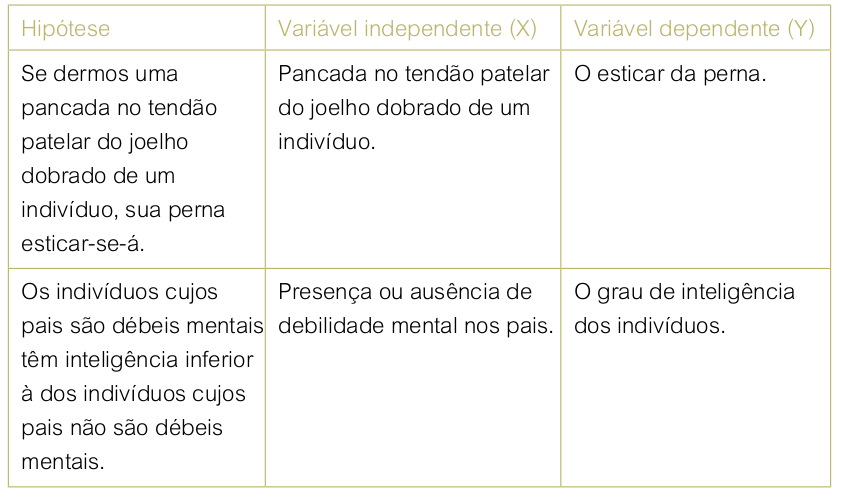
\includegraphics[height=0.8\textheight]{Hipoteses_variaveis/hipotese_variaveis}

  Fonte: Prodanov, 2013
\end{frame}

\section{Formulação sistemática de pergunta - PICO}

\section{Aprofundamento}

\subsection{Aprofundamento}

\begin{frame}{Aprofundamento}
  \begin{block}{Leitura obrigatória}
  \end{block}
  \begin{block}{Leitura recomendada}
    \begin{itemize}
      \footnotesize
    \item Livro texto: seções {\bf 4.1, 4.3, 4.4}
    \end{itemize}
  \end{block}
\end{frame}

\end{document}
